\documentclass{article}
\usepackage[utf8]{inputenc}
\usepackage[margin=1.0in]{geometry}
\usepackage{graphicx}
\usepackage{physics}
\usepackage{siunitx}
\usepackage{bm}
\usepackage{amsmath} 
\usepackage{natbib}
\usepackage{xcolor}

\def\mathunderline#1#2{\color{#1}\underline{{\color{black}#2}}\color{black}}

\title{Running the MITgcm in Slope Coordinates}
\author{Henri Drake}
\date{February 2019}

\begin{document}

\maketitle

\section{Transforming the MITgcm model equations into slope coordinates}\label{appendix}

The MITgcm hydrostatic model equations (with a linear equation of state that depends only on temperature) are given by\footnote{Note that $z \rightarrow r$ and $p \rightarrow \phi$ in the notation used in the documentation of the MITgcm.}
\begin{gather}
    \pdv{u}{t} + \pdv{p_{s}}{x} + \pdv{p_{hyd}}{x} = - \bm{u} \cdot \nabla u -\left\{ -2\Omega v \sin{\varphi} \right\} + \mathcal{F}_{u}
    \\
    \pdv{v}{t} + \pdv{p_{s}}{y} + \pdv{p_{hyd}}{y} = - \bm{u} \cdot \nabla v -\left\{ 2\Omega u \sin{\varphi} \right\} + \mathcal{F}_{v}
    \\
    \pdv{p_{hyd}}{z} = g\alpha \Theta
    \\
    \pdv{\Theta}{t} = - \bm{u} \cdot \nabla \Theta + Q_{\Theta},
\end{gather}
where $\mathcal{F}_{u_{i}}$ are momentum forcing terms, $Q_{\Theta}$ is the temperature forcing, $\varphi$ is the latitude, and we have decomposed the pressure $p = p_{hyd} + p_{s}$ into a hydrostatic component $p_{hyd}$ and a surface component $p_{s}$.

Following \cite{Callies2018RestratificationEddies}, we find it convenient to further decompose the hydrostatic pressure $p_{hyd} = p_{b}(z) + p_{p}(x,y,z)$ and potential temperature $\Theta = \Gamma z + \Theta_{p}(x,y,z)$ into a background component that balances a uniform stratification $\pdv{p_{b}}{z} = g \alpha \Gamma z$ (with lapse rate $\Gamma$) and a perturbation component $\pdv{p_{p}}{z} = g \alpha \Theta_{p}(x,y,z)$. Then, we rewrite the model equations in terms of just the perturbations
\begin{align}
    \pdv{u}{t} + \pdv{p_{s}}{x} + \pdv{p_{p}}{x} &= - \bm{u} \cdot \nabla u -\left\{ -2\Omega v \sin{\varphi} \right\} + \mathcal{F}_{u}
    \\
    \pdv{v}{t} + \pdv{p_{s}}{y} + \pdv{p_{p}}{y} &= - \bm{u} \cdot \nabla v -\left\{2\Omega u \sin{\varphi} \right\} + \mathcal{F}_{v}
    \\
    \pdv{p_{p}}{z} &= g\alpha \Theta_{p}
    \\
    \pdv{\Theta_{p}}{t} &= - \bm{u} \cdot \nabla \Theta_{p} - w\Gamma + Q_{\Theta},
\end{align}
where we have introduced the \ the no-normal flux boundary condition on the potential temperature perturbation becomes $( \nabla \Theta_{p}) \cdot \hat{\bm{n}} = - \Gamma (\hat{\bm{z}} \cdot \hat{\bm{n}})$ with $\hat{\bm{n}}$ normal to the boundary. This formulation allows the velocities and potential temperature perturbations to be periodic in the cross-slope direction while still maintaining a constant background stratification $N^{2} = g \alpha \Gamma$. Taking advantage of this, we now rotate the model equations into slope coordinates $(\hat{x},\hat{y},\hat{z}) = (x\cos{\theta} + z\sin{\theta}, y, z\cos{\theta} - x\sin{\theta})$, where $\theta$ is the slope angle. The model equations in slope coordinates are given by
\begin{align}
    \pdv{\hat{u}}{t} + \pdv{p_{g}}{\hat{x}} + \pdv{p_{p}}{\hat{x}} &= - \hat{\bm{u}} \cdot \nabla \hat{u} - \left\{-2\Omega \hat{v} \sin{\varphi} \right\}\mathunderline{blue}{\cos{\theta}} + \mathunderline{red}{g\alpha \Theta_{p} \sin{\theta}} + \mathcal{F}_{\hat{u}}
    \label{mitgcmrotated1}
    \\
    \pdv{\hat{v}}{t} + \pdv{p_{g}}{\hat{y}} + \pdv{p_{p}}{\hat{y}} &= - \hat{\bm{u}} \cdot \nabla \hat{v} -\left\{2\Omega (\hat{u} \mathunderline{blue}{\cos{\theta}} - \mathunderline{red}{\hat{w}\sin{\theta}}) \sin{\varphi} \right\} + \mathcal{F}_{\hat{v}}
    \\
    \pdv{p_{p}}{\hat{z}} &= g\alpha \Theta_{p}\mathunderline{blue}{\cos{\theta}} - \mathunderline{red}{\mathunderline{red}{\left\{ 2\Omega \hat{v} \sin{\varphi} \right\} \sin{\theta}}}
    \\
    \pdv{\Theta_{p}}{t} &= - \hat{\bm{u}} \cdot \nabla \Theta_{p} - 
    \mathunderline{red}{\Gamma (\hat{w}\cos{\theta} + \hat{u}\sin{\theta})}+ Q_{\Theta}.\label{mitgcmrotated2}
\end{align}
We implement this coordinate transformation by adding the terms underlined in red to the momentum and potential temperature tendencies, adding geometric corrections underlined in blue to existing terms, and adding the term underlined twice in red as a modification to the hydrostatic relation, which is used to diagnose the full pressure field by integrating from the surface to each vertical level.

The boundary condition $( \nabla \Theta_{p}) \cdot \hat{\bm{n}} = - \Gamma (\hat{\bm{z}} \cdot \hat{\bm{n}})$ is imposed by adding a potential temperature tendency in the bottom grid cell equivalent to the effective heat flux across the boundary due to the background stratification.

\section{Model setup}

To test my implementation of the coordinate transformation, I set up two transient experiments, `default' and `rotated', which solve for the evolution of a flow field in response to mixing along a sloping boundary from a state of rest. The domain slopes upwards in the positive $x$ (or $\hat{x}$) direction. The two simulations should have identical evolutions for the spin-up problem, at least until the difference in the cross-slope boundary conditions (periodic versus vertical wall) being to affect the solution. The configurations are both three dimensional ($nz = 200, ny = 128, nx = 128$) with identical grid spacing ($dz \approx 5 \text{ m}, dx = 300 \text{m}, dy = 300 \text{m}$) and timestep $dt=\SI{60}{s}$. In both experiments, the background stratification is $N^{2} = 10^{-6}$ s$^{-2}$ and the mixing coefficients are set to constant $\kappa = \nu = 10^{-3}$ m$^{2}$/s to simplify the comparison between the experiments. The Coriolis parameter is set to $f_{0} = \SI{5.3e-5}{s^{-1}}$ and the slope angle is $\theta = \SI{2e-3}{rad}$.

In the default configuration, there is a discontinuity in the seafloor depth between the left and right boundaries in the $x$ direction due to the existence of a large-scale slope, preventing the boundary condition in $x$ from being periodic. Thus, we instead introduces vertical walls by making the depth go to zero at both $x$ boundaries. This MITgcm configuration reproduces the analytical one-dimensional solution of \cite{Garrett1990TheMixing} for short times (not shown). For longer times, the solution eventually diverges from the one-dimensional solution because of the presence of boundaries in the cross-slope direction and the lack of a buoyancy restoring, which in the one-dimensional problem is provided by cross-slope advection of the background buoyancy.

The advantage of the rotated system of coordinates is that the solution can be made periodic in the cross-slope direction in terms of the perturbations. Unlike the default configuration, buoyancy restoring is then provided by advection of the background stratification and the solution can reach an steady state.

\section{Preliminary results (and lack there-of)}

Figure \ref{rotated_bbl} shows the bottom boundary layer solution at $t = \SI{132}{min}$, a few timesteps before the rotated simulation blows up. Until the solution blows up, the rotated simulation reproduces the analytical one-dimensional solution of \cite{Garrett1990TheMixing} very well, capturing the up-slope and southward flow and warming of the bottom boundary layer. I am still unsure why the solution is blowing up, but row 5 of figure \ref{rotated_bbl} suggests that my current implementation of the additional terms in the cross-slope momentum equation introduces some error. I will be meeting with Jean-Michel Campin to work through my implementation soon.

Despite the fact that my solutions are currently blowing up, the agreement between the two simulations for short times is promising.

\begin{figure}[htb!]
\noindent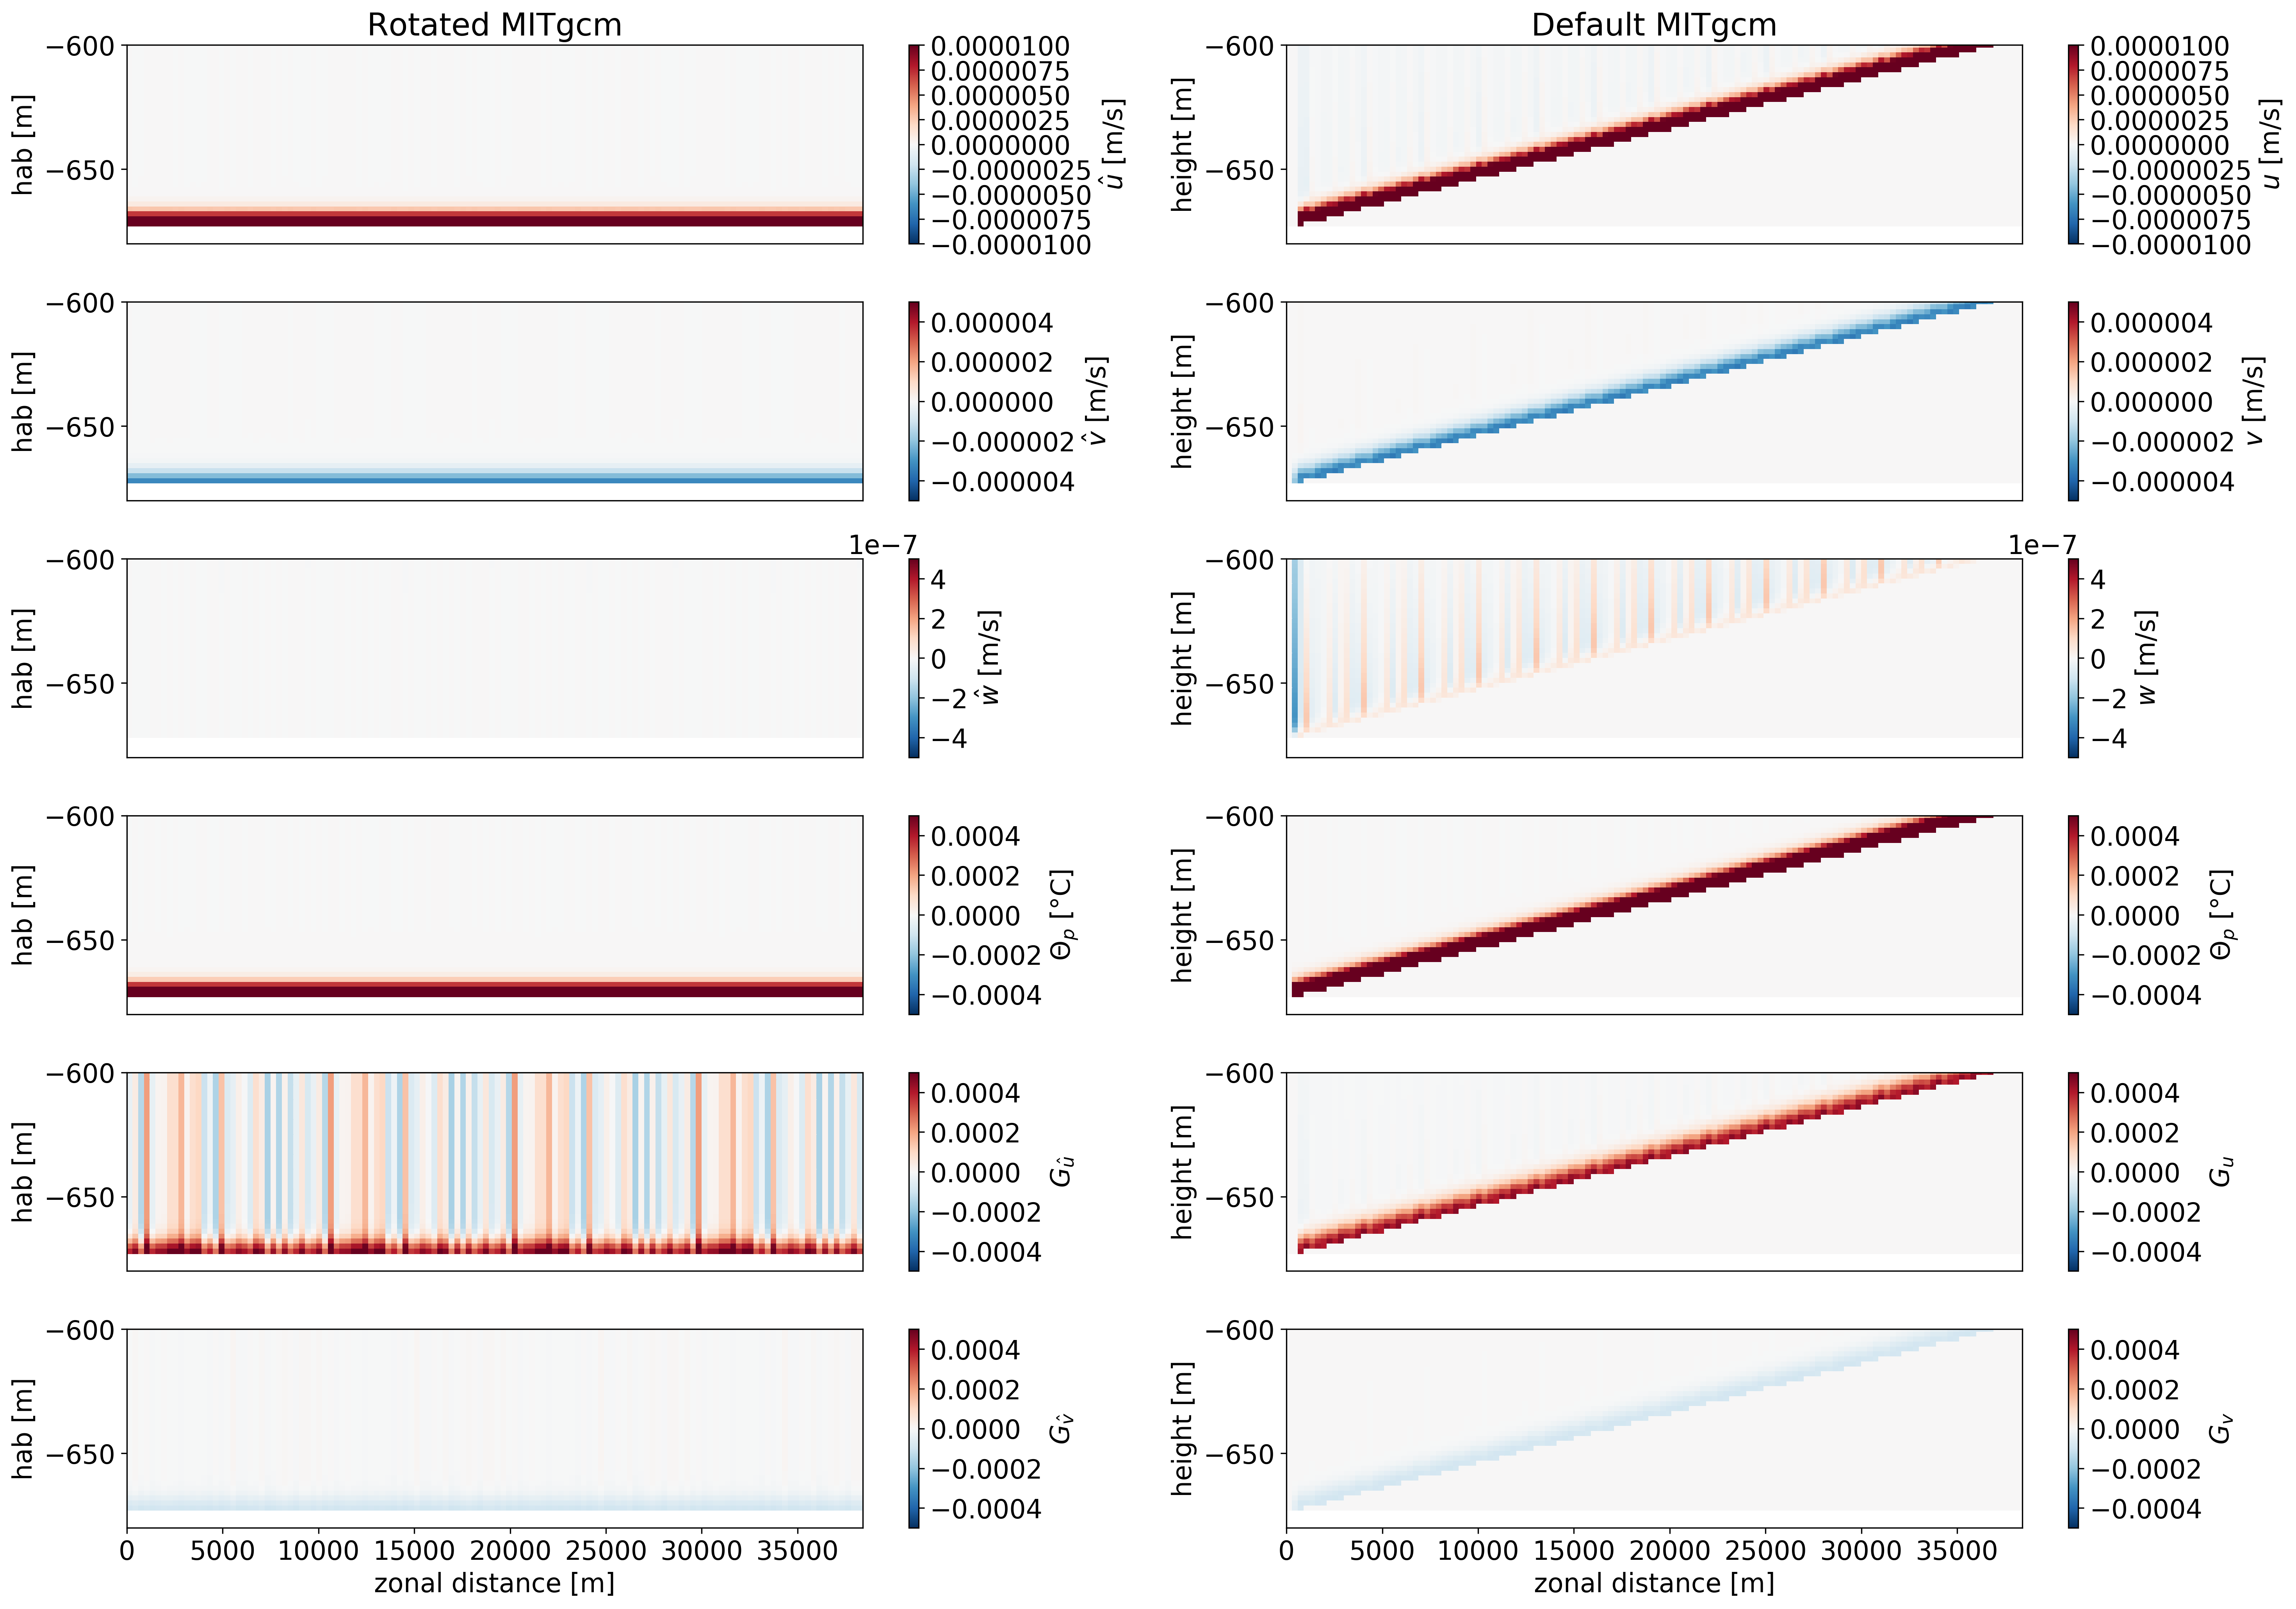
\includegraphics[width=1.0\textwidth]{rotated_bbl.png}
\centering
\caption{Spin-up of the bottom boundary layer on a slope in a rotated, stratified fluid in (left) the MITgcm formulation rotated into slope coordaintes ($\hat{x}$ points up-slope) and (right) the default MITgcm formulation. The first three rows show the three components of the velocity, the fourth shows the temperature perturbation as heat is diffused into the bottom boundary layer, and the bottom two shows show the momentum tendencies for the components in the slope / horizontal planes.}
\label{rotated_bbl}
\end{figure}

\bibliographystyle{apa}
\bibliography{references.bib}

\end{document}

